%
% File naaclhlt2010.tex
%
% Contact: nasmith@cs.cmu.edu

\documentclass[11pt,letterpaper]{article}
\usepackage{naaclhlt2010}
\usepackage{times}
\usepackage{latexsym}
\usepackage{hyperref}
\usepackage{graphicx}
\usepackage{wrapfig}
\usepackage{url}
\usepackage{wrapfig}
\usepackage{color}
\usepackage{marvosym}
\usepackage{enumerate}
\usepackage{subfigure}
\usepackage{tikz}
\usepackage{amsmath}
\usepackage{amssymb}
\usepackage{hyperref}
\usepackage{bbm}

\DeclareMathOperator*{\argmax}{arg\,max}

\setlength\titlebox{4cm}    % Expanding the titlebox


\newcommand{\vwi}{{\bf w}_i}
\newcommand{\vw}{{\bf w}}
\newcommand{\vx}{{\bf x}}
\newcommand{\vy}{{\bf y}}
\newcommand{\vb}{{\bf b}}
\newcommand{\valpha}{{\bf \alpha}}
\newcommand{\vxi}{{\bf x}_i}
\newcommand{\yi}{y_i}
\newcommand{\vxj}{{\bf x}_j}
\newcommand{\vxn}{{\bf x}_n}
\newcommand{\yj}{y_j}
\newcommand{\ai}{\alpha_i}
\newcommand{\aj}{\alpha_j}
\newcommand{\X}{{\bf X}}
\newcommand{\Y}{{\bf Y}}
\newcommand{\vz}{{\bf z}}
\newcommand{\msigma}{{\bf \Sigma}}
\newcommand{\vmu}{{\bf \mu}}
\newcommand{\vmuk}{{\bf \mu}_k}
\newcommand{\msigmak}{{\bf \Sigma}_k}
\newcommand{\vmuj}{{\bf \mu}_j}
\newcommand{\msigmaj}{{\bf \Sigma}_j}
\newcommand{\pij}{\pi_j}
\newcommand{\pik}{\pi_k}
\newcommand{\D}{\mathcal{D}}
\newcommand{\el}{\mathcal{L}}
\newcommand{\N}{\mathcal{N}}
\newcommand{\vxij}{{\bf x}_{ij}}
\newcommand{\vt}{{\bf t}}
\newcommand{\yh}{\hat{y}}
\newcommand{\code}[1]{{\footnotesize \tt #1}}
\newcommand{\alphai}{\alpha_i}

\title{2D Visualizations for Support Vector Machine and Neural Network}

\author{Jizhou Xu \, Aileme Omogbai \\
	Johns Hopkins University \\
	{\tt $\{jxu55, aomogba1\}$@jhu.edu}}

\date{December 10, 2014}

\begin{document}
\maketitle
\begin{abstract}
We present a web-based demo that helps to visualize the operations and results of some machine learning binary classification algorithms. For this project, we have chosen to implement two non-linear methods, namely Support Vector Machines (SVM) and Artificial Neural Networks. This visualization tool is implemented fully in Javascript and so the data collection,  training  and display of the results is done on the client-side. It displays a 2D canvas such that data points can be added with mouse clicks and the decision boundary generated by the algorithm is displayed. The data points correspond to the $(x,y)$ positions of the points clicked on the canvas. There is also provision for adjusting some parameters of the model. The visualization can be found at \url{http://metoerite-j.github.io/Visual-Machine-Learning}.
\end{abstract}

\section{Introduction}

In the field of machine learning, binary classification problems stem from the need to separate a set of data points into two different classes. In the supervised case, we have data that is already separated such that each data point belongs to one of the defined classes. For the unsupervised case, we do not know the classes for the example data available. In both cases, we wish to find a model that can learn parameters for the classification such that new unlabeled data points can be assigned to the right class. The model therefore creates "boundaries" such that a data point is labeled according to the side of the boundary that it falls in. 

If the boundary used to separate the two sets of data points is a line, then the problem is a linear classification problem. The data is not usually linearly separable and so complex functions may be needed to define the boundary. Also, while it is intuitive to visualize the concept of the boundary in 2 dimensions, the data is usually of much higher dimensions. This means that very complex decision boundaries are needed to bring about separation in practical applications. Even in 2D however, it may be difficult to picture the boundary that is generated by non-linear classifiers, and that is what this project aims to help with.

We present a web visualization tool that shows the classification results of two popular non-linear classifiers. The user is presented with a 2D canvas that contains default points that have been generated with a normal distribution and classified randomly. The classes used for the demo are represented by the colors black/white and this used to label the data points and the regions on the canvas. So, a point is labeled either black or white. Also, the color of any position in the canvas represents the class that a test data point (i.e. a point we want to classify) will be assigned to by the current model. Therefore, the boundary between the white and black regions on the canvas represent the decision boundary that was generated by the algorithm used. 

At the current stage, we have implemented two popular non-linear classifiers: Support Vector Machines (SVM) and Artificial Neural Network (ANN). For training the SVM, we used the Primal Estimated Sub-Gradient Solver for SVM (Pegasos) algorithm. For neural networks training, we used the feed-forward back-propagation neural network as our model. 
SVMs are effective and popular classification learning tool. The task of learning a support vector machine is cast as a constrained quadratic programming problem.  stochastic sub-gradians descent algorithm for solving the optimization problem cast by SVMs.

\begin{figure*}
\centering
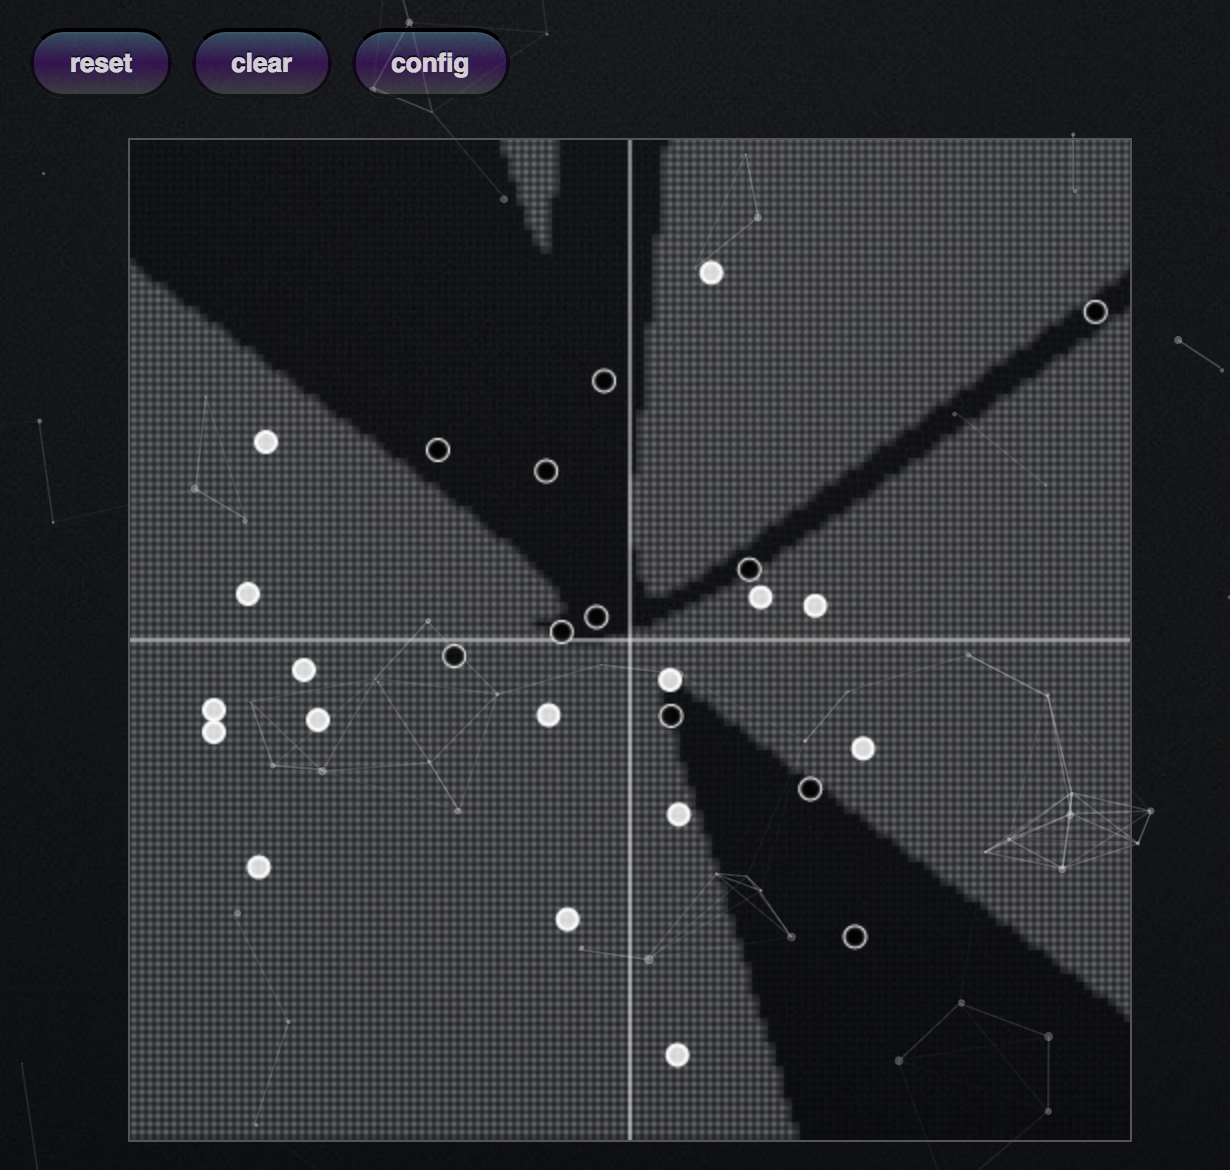
\includegraphics[scale=.5]{images/Intro.PNG}
\caption{Sample output}
\label{fig:intro}
\end{figure*}

\section{SVM}

\subsection{Background}
	The SVM is a very popular model for classification. In the SVM model, data points are seen as points in the $m$-dimensional plane defined by the data. The intuition is that we want to separate the data points with an $(m-1)$-dimensional hyperplane which corresponds to a linear separation. We want to choose the separating line such that its distance to the nearest data point on each side is maximized, which is called maximizing the margin. So we learn the weights in each dimension for that hyperplane. The data points that are closest to the separating hyperplane, that is the data points that affect the position of the hyperplane are called the support vectors. Formally, given a training set $\{(\vxi,\yi)\}_{i=1}^N$, where $\vx_i \in \mathbb{R}^M$ and $y_i \in\{+1,-1\}$, we want to solve the constrained the problem:
\begin{align}
\argmax_{\valpha >= 0} \min_{\vw,b} \{ \frac{1}{2} ||w||^2  - \sum_i^N \alpha_i\left[\yi(\vw \vx - b) - 1\right]  \}
\end{align}
where $b$ is the bias term that determines the offset of the hyperplane from the origin, $w$ denotes the normal vector to the hyperplane and $\alpha$ are Lagrange multipliers. This equation is known as the primal formulation of the optimization problem.

What makes SVMs very popular is that they can be made into non-linear classifiers by applying the "kernel trick". The algorithm is essentially the same except that the dot product used to compute the margins is replaced with a kernel function that represents a dot product also, but in a higher dimension. In this project, we used the radial basis function (RBF) kernel to separate non-linearly separable data.

%\begin{figure*}
%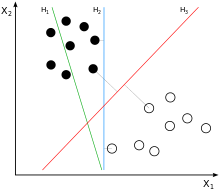
\includegraphics[scale=1]{images/Svm_separating_hyperplanes.PNG}
%\caption{SVM margins [Wikipedia]}
%\label{fig:svm}
%\end{figure*}
\subsection{Training}
There are different algorithms for training SVMs like:
\begin{enumerate}
\item
the Sequential Minimal Optimization (SMO), and
\item
Primal Estimated sub-GrAdient SOlver for SVM (Pegasos).
\end{enumerate} 

We chose to implement the Pegasos algorithm for training the SVM in this project. The basic algorithm involves using stochastic gradient descent to solve the primal formulation of the problem in $w$ which corresponds to the linear SVM. However, as explained  in $•$, the algorithm can also be modified to handle the non-linear kernelized case as well. See the paper for more information on the algorithm. We have implemented both versions of the algorithm, so the user can try both the linear and kernel forms to see the boundaries generated by each model type. The application also makes it possible for the user to generate synthetic linearly separable data in order to see the linear SVM solution better. 

\subsection{Implementation}
The implementation of the SVM visualization is divided into two sections. This applies to the other models as well. The actual implementation of the Pegasos algorithm is in a js file that is separate from the actual visualization page. That file thus contains the code for training the SVM, predicting the class of points after training and all other functions necessary for the training algorithm to work. The usage is as follows:
\begin{enumerate}[i]
\item
Create a new instance of the Pegasos trainer: $pegasos.SVM$.
\item
Call the $train$ method, passing in the data points, the labels and the options for training. Some of the options include: the value of $\lambda$ used in the Pegasos algorithm, number of iterations to be run, the type of kernel ("linear" for linear SVM, and for now "rbf" for RBF kernel), and the value of $\sigma$ for the RBF kernel.
\item
After training, call $predictOne$ to predict a specific data point, or $predict$ for a set of points.
\end{enumerate}
The linear and kernelized versions of the Pegasos are quite different and so they are implemented separately and used depending on which is specified in the training options. For the linear case, the model parameters are the $w$ values but in the kernelized version, its easier to keep the parameters as $\alpha$, the Lagrangian multipliers. These values are used to predict the class of points after training.

The visualization page calls the training algorithm and displays the results on the canvas. Once the page is loaded, default data points corresponding to points on the canvas are generated from a Gaussian distribution and classified arbitrarily. The data is used to train the model. For drawing the data points, boundaries and many finicky details of 2D drawing with Javascript, we made use of a library written by Andrej Karpathy $•$. To display the decision boundary, we predict the class of every point on the canvas. The boundary is seen as the separation between the white and dark regions on the canvas.

The user is able to switch from a linear SVM to using a kernel and the model is retrained appropriately and the decision boundary displayed. For the linear SVM, we show the decision boundary and the margins of the classifier. Because the default data generated is not likely to be linearly separable, we provided an option to clear the points and input new data points. This can be used to generate linearly separable data, because the linear classifier will not produce sensible boundaries for non-linear data.

It is also possible to vary the value of the parameter of the RBF kernel $\sigma$, which has a big effect on the shape of the decision boundary. By the definition of the kernel, small values of $\sigma$ will make it such that only points close to each other will affect prediction because the value of the kernel will be close to zero for points far from each other. The model will look to be overfitting the data. For large values of $\sigma$, we get smooth boundaries that mis-classifies points, tending towards a linear classifier.

\section{SMO}

\subsection{Background}

SMO is one of the most popular algorithms for training SVMs. It tackles the dual representation of the SVM optimization problem, and employs an active set of constraints thus working on a subset of dual variables. Normally, training a Support Vector Machine (SVM) requires the solution of a very large quadratic programming (QP) optimization problem. SMO breaks this large QP problem into a series of smallest possible QP problems. These small QP problems are solved analytically, which avoids using a time-consuming numerical QP optimization as an inner loop. The amount of memory required for SMO is linear in the training set size, which allows SMO to handle very large training sets. Because large matrix computation is avoided, SMO scales somewhere between linear and quadratic in the training set size for various test problems, while a standard projected conjugate gradient (PCG) chunking algorithm scales somewhere between linear and cubic in the training set size. SMO's computation time is dominated by SVM evaluation, hence SMO is fastest for linear SVMs and sparse data sets.

The full SMO algorithm contains many optimizations designed to speed up the algorithm on large datasets and ensure that the algorithm converges even under degenerate conditions. The SMO we present is a much simpler version.




\begin{figure}
%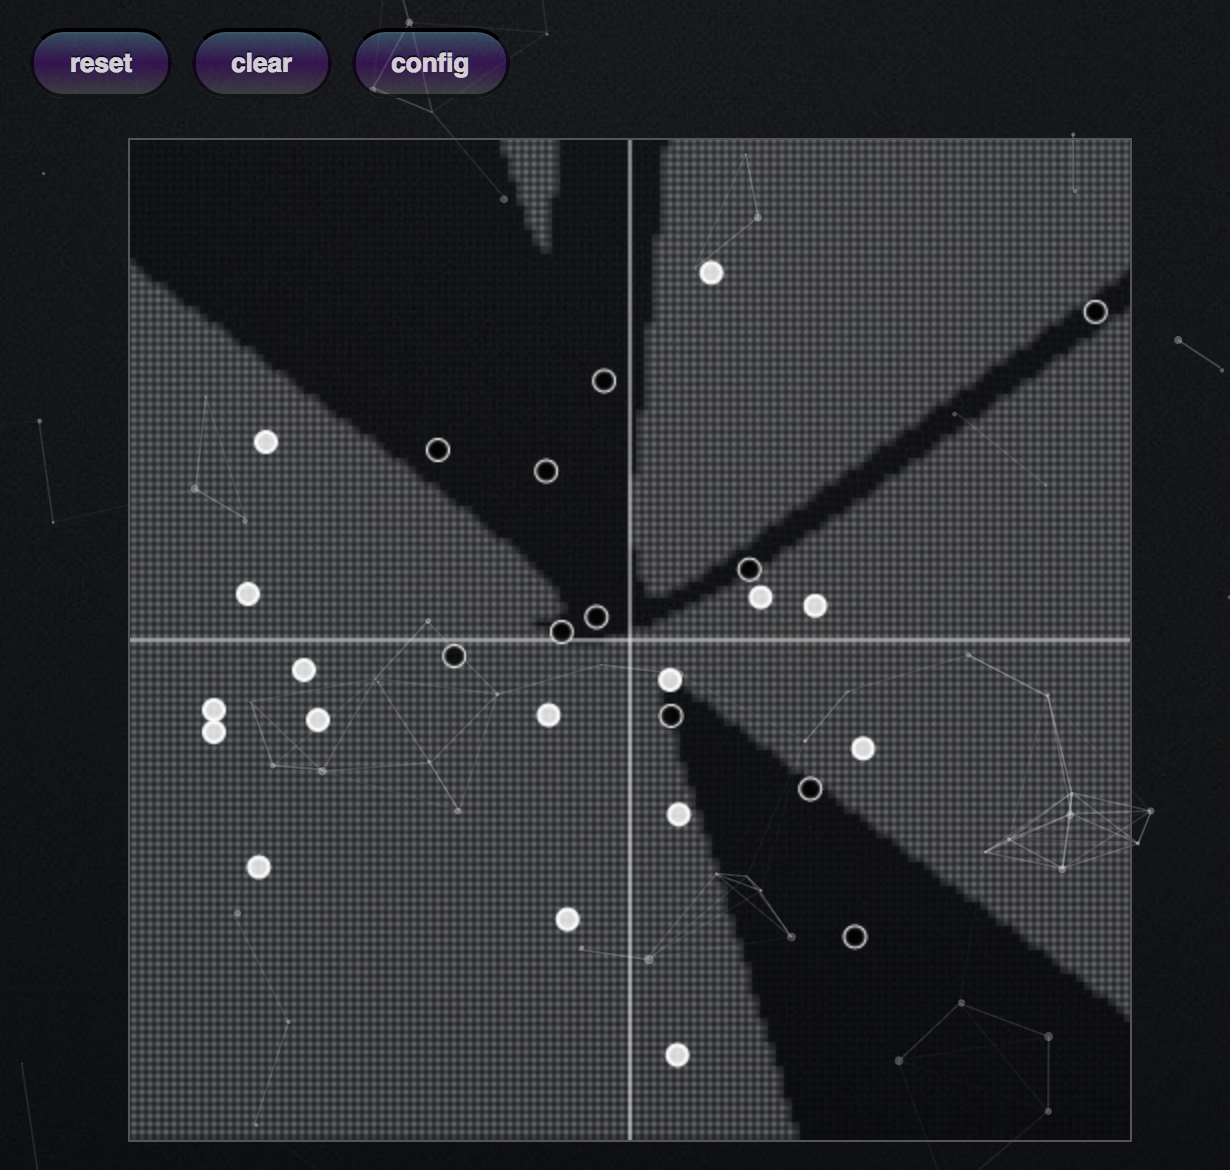
\includegraphics[scale=.1]{images/Intro.PNG}
%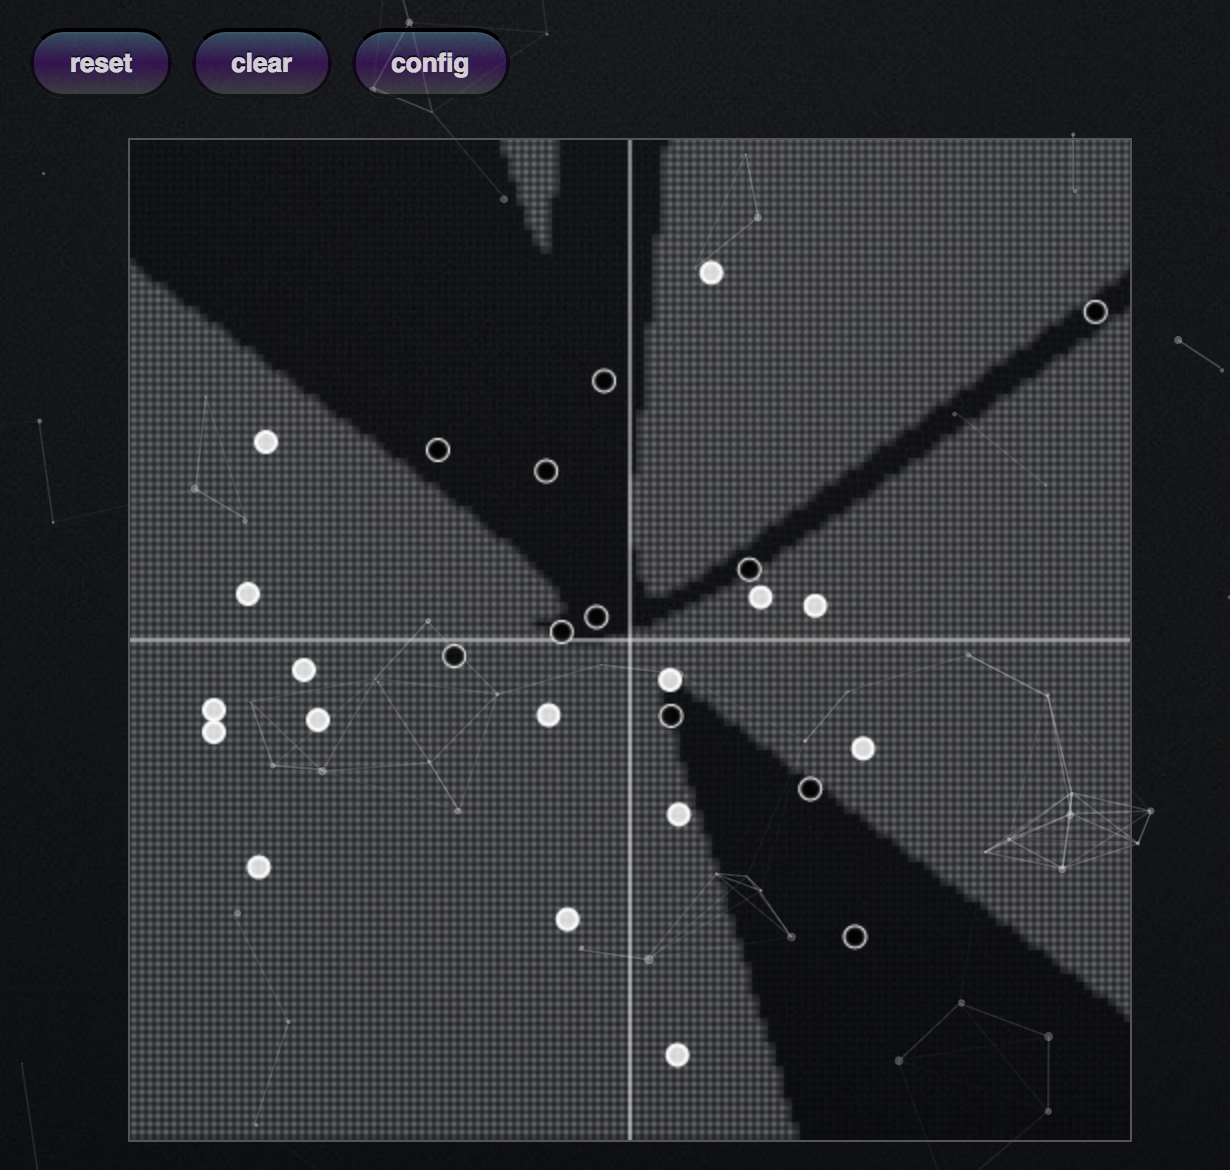
\includegraphics[scale = .1]{images/Intro.PNG}
\fbox{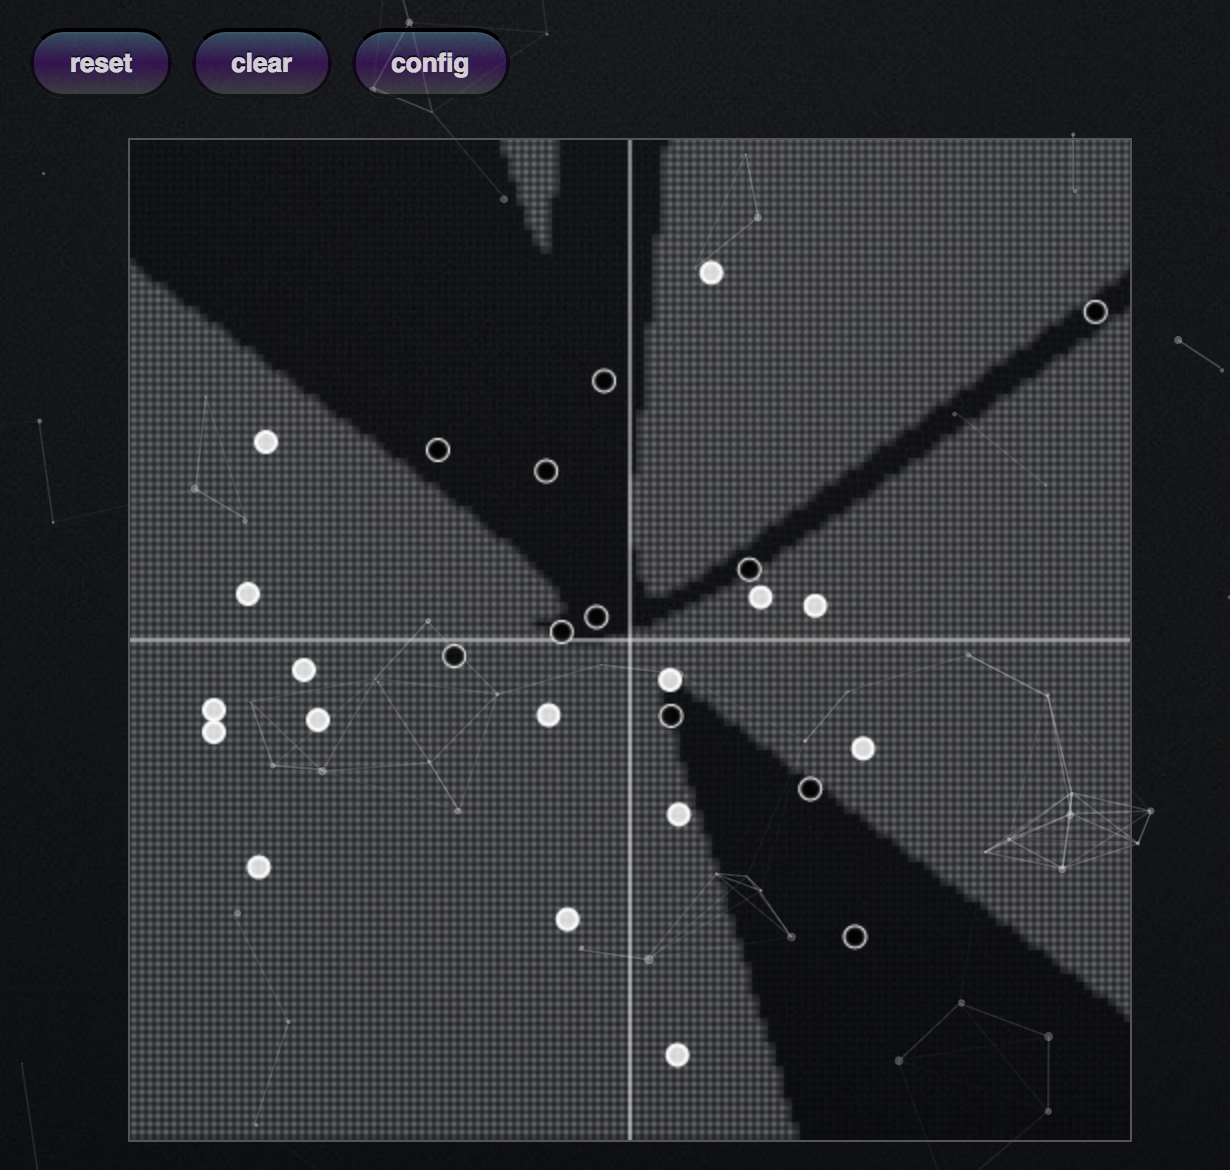
\includegraphics[scale=.3]{images/Intro.PNG}}
\caption{Sample output}
\label{fig:intro}
\end{figure}
\section{ANN}

\subsection{Background}

In machine learning, ANNs are a family of statistical learning algorithms and are used to estimate or approximate functions. An Artificial Neural Network (ANN) can be regard as an information processing paradigm that is inspired by the way biological nervous systems, such as the brain, process information.  The key element of this paradigm is the novel structure of the information processing system. It is composed of a large number of highly interconnected processing elements ("neurons") working in unison to solve specific problems. ANNs, like people, learn by example. Learning in biological systems involves adjustments to the synaptic connections that exist between the neurons, and this is true of ANNs as well. Simulations of ANNs appear to be a recent development. However, this field was established before the advent of computers, and has survived at least one major setback and several eras.

Neural networks are remarkable when it comes to derive meaning from complicated (sometimes imprecise) data. They are often used to detect trends and extract patterns that are too complex to be noticed by normal algorithms. They have an ability to learn how to do tasks based on the data given for training or initial experience. Also, ANN computations can be carried out in parallel, and special hardware devices are being designed to take advantage of this. Modern applications of ANNs are various, such as classification, data processing (clustering, filtering...), regression analysis, etc. We are going to introduce one of the easiest neural networks - the feedforward neural network.

A neural network is created by hooking together many of the "neurons" we've introduced. Each of the neurons usually have multiple inputs and one output. The commonest type of artificial neural network consists of three layers of such neurons: a layer of "input" units is connected to a layer of "hidden" units, which is connected to a layer of "output" units.

\subsection{Implementation}
\label{sect:pdf}
We adjust the weights of the neural network to minimize the mean squared error (MSE) on training set.
$$\underset{min}{arg} (MLE = \frac{1}{n}\sum_{i=1}^n(y_i^*-y_i)^2)$$
For each neuron:\\\\
\textbf{Initialization:}\\
weights: $w$ = rand(0, 1)\\
bias: $b$ = rand(0, 1)\\
mean squared error: $MLE$ = 0\\
output: $y$ = 0\\\\
\textbf{Train:}\\
Compute output: \\
$sum = \boldsymbol{w}\times \boldsymbol{y},$\\
where $\boldsymbol{y}$ is the vector containing the outputs from the previous layer.\\
$sum = sum + bias$\\
$y = sigmoid(sum)$\\
Compute Error: $e = y* - y$\\
Update Weights:
$$w' = w + \eta *\frac{\alpha (MLE)}{\alpha w},$$
where $\eta$ is the learning rate.\\\\
\textbf{Predict:}\\
$decision = (y > 0.5) ? 1:0$

\subsection{Result}
The default configuration of out neural network is 2-10-10-1: 2 inputs (x and y coordinates), 2 layers of 10 hidden neurons each, and
\section*{Acknowledgments}


% Up to two (2) additional pages may be purchased from ACL at the
% price of \$250 per page; please contact the publication chairs above
% for more information about this option.

\section*{Acknowledgments}

Do not number the acknowledgment section.

\begin{thebibliography}{}

\bibitem[\protect\citename{Aho and Ullman}1972]{Aho:72}
Alfred~V. Aho and Jeffrey~D. Ullman.
\newblock 1972.
\newblock {\em The Theory of Parsing, Translation and Compiling}, volume~1.
\newblock Prentice-{Hall}, Englewood Cliffs, NJ.

\bibitem[\protect\citename{{American Psychological Association}}1983]{APA:83}
{American Psychological Association}.
\newblock 1983.
\newblock {\em Publications Manual}.
\newblock American Psychological Association, Washington, DC.

\bibitem[\protect\citename{{Association for Computing Machinery}}1983]{ACM:83}
{Association for Computing Machinery}.
\newblock 1983.
\newblock {\em Computing Reviews}, 24(11):503--512.

\bibitem[\protect\citename{Chandra \bgroup et al.\egroup }1981]{Chandra:81}
Ashok~K. Chandra, Dexter~C. Kozen, and Larry~J. Stockmeyer.
\newblock 1981.
\newblock Alternation.
\newblock {\em Journal of the Association for Computing Machinery},
  28(1):114--133.

\bibitem[\protect\citename{Gusfield}1997]{Gusfield:97}
Dan Gusfield.
\newblock 1997.
\newblock {\em Algorithms on Strings, Trees and Sequences}.
\newblock Cambridge University Press, Cambridge, UK.

\end{thebibliography}

\end{document}
